\documentclass[conference]{IEEEtran}

\ifCLASSINFOpdf
   \usepackage[pdftex]{graphicx}
   \graphicspath{{../pdf/}{../jpeg/}}
\else
\fi

\usepackage[cmex10]{amsmath}

\usepackage[tight,footnotesize]{subfigure}

\usepackage{booktabs}

\begin{document}

%\title{Deriving Actionable Knowledge from Information on Socio-Technical Gaps in Software Projects}

\title{Deriving Actionable Knowledge from Socio-Technical Gaps in Developer Coordination}

%On Socio-Technical Coordination and its Relation to Build Failure}


\author{\IEEEauthorblockN{Adrian Schr{\"o}ter}
\IEEEauthorblockA{University of Victoria, Canada\\
schadr@acm.org}
\and
\IEEEauthorblockN{Daniela Damian}
\IEEEauthorblockA{University of Victoria, Canada\\
danielad@cs.uvic.ca}}

\maketitle

% MKAE IT TALK ABOUT THE APORACH AND NOT CASE STUDY

\begin{abstract}
The misalignment between the social and technical dimensions of software development has been
linked to losses in developer productivity and increases the likelihood of a build to fail. Although research has produced empirical evidence of this relationship, it has yet to produce actionable knowledge that managers and developers can act upon to avoid build failure.
We propose an approach that generates recommendations to alleviate the effect that mismatches between the social and technical dimensions of a software project has on  builds failure. Specifically, our approach analyzes the technical dependencies, actual coordination and all builds in a project, and recommends a ranked list of developer pairs that, if present in the current build, will increase the current build's chance of failure. We discuss our preliminary evaluation of our approach using data from the IBM Rational Team Concert\texttrademark\ project and outline future steps in our research. 


%showed that we can recommend pairs of developers that form the mismatch between the social and technical dimensions.
%These pairs were statistically related to build failure and offer to managers and developer opportunities to improve the chance that the current build will succeed.
%Two developers that form a mismatch can improve the alignment between the social and technical dimensions by initiating coordination.
%
%
%
%In a case study of
%coordination in the IBM Jazz\texttrademark\ project, we investigate the
%communication and technical dependencies between developers involved in
%software builds and relate their misalignment to the build failure.  
%Through our proposed approach we identified a number of developer pairs that did not communicate  their dependencies and thus increased the likelihood of build failure. 
%Upon this actionable knowledge, developers and managers can act to prevent build failure. 
%If any one of these pairs is present in a build's social network, the build had at least a 74\% chance to fail. 
%This has several practical implications for the design of collaborative systems, such as the integration of recommendations about inter-personal relationships.
\end{abstract}

\IEEEpeerreviewmaketitle

\section{Introduction}
A growing body of research (e.g. ~\cite{kwan:tse:2011,herbsleb:icse:1999}) shows that with the ever growing size of software teams the lack of
effective coordination is the main source of integration failures. The
development work that precedes integrations involves significant coordination of
developers that work in teams and need to rely on the code of others. 
Unfortunately, code is often anything but stable, further contributing to developers' need to coordinate with one another and stay up to date with code changes that impact their work.
%But often code is everything but stable, further contributing to
%developers' needing to coordinate to keep up with code changes that impact their work. 
This problem is
amplified in software builds that integrate an entire team's work
and on which the delivery of new features depends. Not only do
failed builds destabilize the product~\cite{cusumano1997}, they also demotivate
software developers~\cite{holck2004}.

%Keeping integrations builds error-free can be a very time consuming
%process. 
One major challenge with integrating work across teams is coordination~\cite{cataldo:esem:2008}.
Coordination problems can arise from factors of organizational,
social or technical nature~\cite{herbsleb:icse:1999}. Studies showed that the mismatch between technical dependencies and required communication to tackle these dependencies increases the likelihood of integration failures~\cite{kwan:tse:2011}. Similarly, research~\cite{wolf:icse:2009,hassan:ase:2006} trained predictive models to assess the quality of software builds without the need to invoke large test suits. Although this research
reaches a high degree of accuracy in their predictions, knowing that a
build will fail or that failures happen due to socio-technical mismatches does not necessarily help developers to prevent the build from failing. Pinpointing more precise build-related coordination problems enhances a team's ability to devise strategies to avoid build failure. 



%relate to build failure is even more important for a team's
%ability to devise strategies to avoid this problem.
%Thus an approach to support developers to identify co-workers they need to coordinate with in order to avoid the up coming build from breaking is called for.
%Thus it is important to initiate an approach that supports developers in identifying coworkers that they need to coordinate with in order to avoid an up coming build from breaking.


%The goal of this research is to find a way to create actionable knowledge to avoid
%integration failure.

Our research seeks to identify actionable knowledge to avoid integration failure by providing developers with information with which coworkers they need to coordinate with in order to avoid failure of the upcoming build. In this paper we describe an approach that we evaluated with data from the IBM's Rational Team Concert project in which we leverage
information about socio-technical developer coordination and software builds to
identify pairs of developers that increase the likelihood of a build failing. From historical project information we extract information about developers with technical dependencies
as well as their ongoing coordination. From this, certain pairs of developers that have a negative influence on the build outcome are identified. This
actionable knowledge can be integrated in real-time recommender systems and developers and management can
devise strategies to prevent failure before build time.

%Through the application of our proposed approach we uncover the existence of pairs of
%developers that if technically dependent in a build but not discussing their
%dependencies, have a negative influence on build success. 

Our approach is based on the hypothesis that due to the high coordination needs in a build the absence of corresponding coordination increases the likelihood of build failure. 
Thus, we
investigate pairs of developers that share a technical dependency in the absence of actual coordination (referred to as \emph{technical pairs}) and formulate our research question:

\textbf{RQ} How can we identify developer pairs that negatively influence build success?
 

\section{Related Work}
\label{sec:relwork}
We aim to integrate work that investigates team collaboration to produce actionable knowledge upon which developers can act.
Several studies are relevant with respect to different dimensions of our work:

\paragraph{Factors that affect software builds}
To the best of our knowledge the studies by Hassan et al.~\cite{hassan:ase:2006}
and Wolf et al.~\cite{wolf:icse:2009} are the only studies that conducted
research to predict build outcome. Hassan et al.~\cite{hassan:ase:2006} found
that a combination of social metrics (e.g. number of authors) and technical
metrics (e.g. number of code changes) derived from the source code repository
yield to be best predictor. 
On the other hand Wolf et al.~\cite{wolf:icse:2009} showed that communication structure has an influence on the build outcome.
Kwan et al~\cite{kwan:tse:2011} investigated socio-technical networks with an emphasis on technical dependencies among developers that is not accompanied with any coordination activity on build outcome (socio-technical gap).
We complement the work of Kwan et al's ~\cite{kwan:tse:2011} that showed a relationship between the number of gaps and build failure, by leveraging information about these gaps to create actionable knowledge.

\paragraph{Coordination in software development}
In order to manage changes and maintain quality, developers must coordinate. In
software development, coordination is largely achieved by communication with those sharing work dependencies~\cite{kraut1995:coordination}. 
The software engineering literature is recognizing the role of communication as essential~\cite{nakakoji2010:rdc}.
Several researchers in the software engineering community investigated the effects of communication on several topics such as knowledge distribution~\cite{ehrlich:icgse:2006}, coordination~\cite{hinds:cscw:2006}, and Conway's Law~\cite{cataldo:cscw:2006}.
We build onto these findings in devising an approach that improves team communication.


\paragraph{Coordination and failure in software development}
Many studies bring evidence of the relationship between coordination and software integrations. Besides qualitative studies (e.g~\cite{herbsleb:icse:1999}), quantitative approaches often represent coordination among developers in the form of social networks. These social networks, when related to actual code artifacts, can be used to predict the artifacts' failure-likelihood.
Several studies showed that metrics derived from social networks form good failure predictors (e.g.~\cite{meneely:fse:2008}).
Furthermore, when combining these social networks with information of organizational hierarchies~\cite{nagappan:icse:2008}, or geographical distance~\cite{bird:acm:2009}, they yield not only better predictors but also shine a light on other factors that influence developers' coordination.
% herbsleb grinter
%Herbselb and Grinter~\cite{herbsleb:icse:1999} found that coordination impacts integration efforts.
%We take the findings that show the influence of coordination on software quality and combine them with technical dependencies among developers to generate actionable knowledge.

Recent work has studied the effects of socio-technical alignment on coordination and project outcomes. The mismatch between coordination needs and actual coordination -- implied by work dependencies and developer social interactions respectively -- is referred to as a socio-technical gap. Empirical studies related socio-technical gaps to low developer productivity~\cite{valetto:msr:2007} and low software quality~\cite{kwan:tse:2011}.
With respect to software builds, Kwan et al~\cite{kwan:tse:2011} investigated the occurrence of socio-technical gaps throughout builds in the Rational Team Concert project highlighting that builds that contain more gaps are more likely to fail.
%Valetto et al~\cite{valetto:msr:2007} uncovered a similar insight into productivity related to implementing work items showing that the existence of gaps is a major cause for low productivity.
These findings suggest that the mismatch between implied coordination needs and actual coordination should be avoided to both guarantee high productivity and software quality.
  

%MOVE THOSE DOWN
%A gap is represented by two developers that share a technical dependency (implying coordination need) without any social interaction (implying
%unmet coordination need).
%In this paper, we refer to these pairs of developers as \emph{technical pairs} (there is a gap), and to those that do
%share a socio-technical dependency (there is no gap) as \emph{socio-technical pairs}.


%MOTIVATE THE APPROACH
%
%WHAT IS THE GOAL OF THE APPROACH
%
%WHAT TYPE OF PROJECTS ARE YOU APPLYING THIS TO
%
%EXAMPLE FOR TECHNICAL PAIRS, HOW DO I BUILD THOSE

\section{Formulating the Approach}
Motivated by research showing that socio-technical gaps increases the chance of a build to fail we formulate an approach that generates actionable knowledge to alleviate socio-technical gaps.
Our approach takes into account the past history of a project analyzing socio-technical gaps with respect to their individual relation to build failure.
These recommendations aim at initiating coordination between two developers that form a gap in the current build, thus increasing the chance of a build to succeed.
This approach can support projects that use electronic repositories such as automated build engines, version control and task management.

For our approach we define a socio-technical gap as the relationship between two developers that share a technical dependency (implying coordination need) without any social interaction (implying unmet coordination need).
A technical dependency can be inferred by two developers changing the same file, or a developer changing a method that another developer's code is calling.
%In this paper, two developers that share a technical dependency are referred to as a \emph{technical pair} (or socio-technical gap).
In contrast two developers that share a technical dependency and that also coordinate their work are referred to as being in a \emph{socio-technical pair}.
For example, two developers that discuss their work through email are said to coordinate; if they additionally share a technical dependency then they form a socio-technical pair.
%
When analyzing the developer pairs in a project's set of builds, in our approach we recognize that each \emph{technical} pair can have a \emph{corresponding socio-technical} if the same two developers have a technical dependency matched by actual coordination in a different build. 

%two developers that are in a technical pair in some builds can also have a \emph{corresponding socio-technical} relationship in a different build (i.e. where their technical dependency is met by actual coordination). 

%We further define a technical and a socio-technical pair to be \emph{corresponding} if both pairs consist of the same pair of developers.

Our approach analyzes the technical pairs in relation to build failure in the following steps:

\begin{enumerate}
\item Identify the set of all technical pairs $T$ across all builds in the project.

\item From set $T$, select the set of \emph{harmful} pairs $H$ by identifying those technical pairs that are statistically related to build failure. To determine the statistical relationship we employ a Fisher exact value test that comparing the frequency of each technical pair's occurrence in failed vs successful builds. The p-values of the Fisher Exact Value test should be adjusted to account for multiple hypothesis testing.

%by counting for each technical pair in how many failed and successful builds it occurs.

\item To form our set of recommendations $R$  we remove from $H$ those pairs where the corresponding socio-technical pair is statistically related to failure ($H_f$) (which would indicate that even matching the technical dependency with actual coordination would not prevent the build from failing). 

Therefore $R = H - H_f$.


%From the set of harmful pairs  (S) we then remove those pairs that have a \emph{corresponding} socio-technical pair that is statistically related to build failure (using a Fisher exact value test as above) forming the set of recommendations.

\item Having identified $R$, we further refine our recommendation by identifying two sets of technical pairs: $R_1$ contains the pairs that have a corresponding socio-technical pair that relates statistically to success and $R_2$ contains the pairs that either (1) have a corresponding socio-technical pair that does not relate to success or failure, or (2) do not have a corresponding socio-technical pair.

Therefore, $R = R_1 \cup R_2$.

In our recommendation the $R_1$ set has highest priority because it contains developer pairs that contributed to a successful build when matched by actual coordination.  

%We split the set of recommendations into two sets of recommendations.
%The first set contains those which have a corresponding socio-technical pair that is statistically related to build success (using a Fisher exact value test as mentioned earlier) whereas the second set contains the remaining technical pairs.

\item Finally, for each set in our recommendation $R$ ($R_1$ and $R_2$) we rank the developer pairs using the coefficient $p_x$, which represents the normalized likelihood of a build
to fail in the presence of the specific pair:
$$
p_x\text{=}\frac{ \text{pair}_{failed} / \text{total}_{failed} }
                     { \text{pair}_{failed} / \text{total}_{failed} + \text{pair}_{success} / \text{total}_{successs}}
$$
where: pair$_{failed}$ is the number of failed builds in which the pair occurred; total$_{failed}$ is the number of failed builds; pair$_{success}$ is the number of successful builds in which the pair occurred, and total$_{success}$ is the number of successful builds.
A value of $p_x$ closer to one means that the developer pair is strongly related to build
failure. 
\end{enumerate}

In summary, our approach analyzes the technical dependencies, actual coordination and build quality in all existing builds in the project, and recommends a ranked list of developer pairs that, if present in the current build, will increase the current build's chance of failure. This list is prioritized by the probability of this chance. This recommendation essentially represents the pairs of developers that should communicate in order to increase the chance of a build to succeed. In a busy manager's workday, the ranking of each developer pair is useful in prioritizing which socio-technical gaps should be closed first. 

%produces two sets of recommendations ($S_1$ and $S_2$) both containing technical pairs that are related to build failure.
%$S_1$ consists of technical pairs that have an equivalent socio-technical pair that is related to build success.
%$S_2$ consists of technical pairs that do not have an equivalent socio-technical pair that is related to either build outcome.
%Both sets of technical pairs represent recommendations of pairs of developers that should communicate in order to increase the chance of a build to succeed. 
%The technical pairs contained in $S_1$ have a potentially larger influence on increase build success due to converting a build failure related pair into a build success related pair.




% !TEX root = develop_pairs_short.tex
\section{Preliminary Evaluation}
To evaluate our approach we analyzed collaboration and build data in the IBM Rational Team Concert\texttrademark\ (RTC) development team.
RTC is a product that integrates source code management, agile planning, and issue management into a single server/client application that the team itself uses for development.
RTC allows developers to link changes they made directly to work items, thus establishing within their repository traceable links between builds and work items through the changes they made.
The repository spans three months in which the team started 326 builds, 99 of which failed and 227 that were successful. 
The team consists of more than 100 developers distributed across seven major sites in Europe, Asia, and North America. Due to the team's geographical distribution and agile development process the team's  communication is largely found in the online repository in the form of comments related to work items. 


In RTC we conceptualize a \emph{technical pair} as two developers that modified the same file in a build.
Similarly, two developers are in a \emph{socio-technical pair} if they modified the same file in a build \emph{and} commented on a work item that was linked to the build in which they changed the same file.

\begin{table}[t]
\centering
%\subtable[Twenty most frequent \emph{technical pairs} that are failure-related.]{
\begin{tabular}{@{\hspace{.2cm}}ccc@{\hspace{.75cm}}c@{\hspace{.2cm}}}
\toprule
Pair & \#successful & \#failed & $p_x$\\
\midrule
%Cody-Daisy&  0 & 12 & 1.0000 \\
%Adam-Ina & 0 & \phantom{1}8 & 1.0000 \\
%Adam-Kim& 0 & \phantom{1}8 & 1.0000 \\
%Adam-Nina & 0 & \phantom{1}6 & 1.0000 \\
%Fred-Gina& 0 & \phantom{1}6 & 1.0000 \\
%Gina-Oliver & 0 & \phantom{1}6 & 1.0000 \\
%Adam-Daisy& 1 & 14 & 0.9720\\%67 \\
%Bart-Daisy& 1 & \phantom{1}9 & 0.9572\\%127 \\
%Adam-Lisa& 1 & \phantom{1}8 & 0.9521\\%204 \\
%Bart-Eve & 2 & 11 & 0.9318\\%403 \\
%\textbf{Adam}-\textbf{Bart}& \textbf{3} & \textbf{13} & \textbf{0.9150}\\%485 \\
%Bart-Cody & 3 & 13 & 0.9150\\%485 \\
%Adam-Eve & 4 & 16 & 0.9086\\%162 \\
%Daisy-Ina & 3 & 12 & 0.9086\\%162 \\
%Cody-Fred& 3 & 10 & 0.8923\\%077 \\
%Bart-Herb & 3 & 10 & 0.8923\\%077 \\
%Cody-Eve & 5 & 15 & 0.8817\\%568 \\
%Adam-Jim & 4 & 11 & 0.8723\\%792 \\
%Herb-Paul & 5 & 12 & 0.8564\\%397 \\
%Mike-Rob& 6 & 13 & 0.8434\\%004\\
%Adam-Fred & 6 & 13 & 0.8434\\%004\\
%
%User11137, User4105 & 0 & 12 & 1.0000 \\
%User2943, User13877 & 0 & 8 & 1.0000 \\
%User7438, User2943 & 0 & 8 & 1.0000 \\
%User2943, User2810 & 0 & 6 & 1.0000 \\
%User8645, User1976 & 0 & 6 & 1.0000 \\
%User8645, User2267 & 0 & 6 & 1.0000 \\
%User11137, User2943 & 1 & 14 & 0.9675\\%908 \\
%User11137, User3493 & 1 & 9 & 0.9504\\%773 \\
%User6012, User2943 & 1 & 8 & 0.9446\\%298 \\
%User3493, User2435 & 2 & 11 & 0.9214\\%387 \\
%User3493, User2943 & 3 & 13 & 0.9023\\%53 \\
%User3493, User4105 & 3 & 13 & 0.9023\\%53 \\
%User2943, User2435 & 4 & 16 & 0.8950\\%695 \\
%User11137, User13877 & 3 & 12 & 0.8950\\%695 \\
%User1976, User4105 & 3 & 10 & 0.8766\\%716 \\
%User3493, User6339 & 3 & 10 & 0.8766\\%716 \\
%User4105, User2435 & 5 & 15 & 0.8648\\%208 \\
%User2943, User9017 & 4 & 11 & 0.8543\\%22 \\
%User6339, User13875 & 5 & 12 & 0.8365\\%498 \\
%User10979, User3385 & 6 & 13 & 0.8220\\%793\\
%User2943, User1976 & 6 & 13 & 0.8220\\%793 \\
%
(Cody, Daisy)	&	0&	12&	1		\\ %user11137.user4105.T
(Adam, Daisy)	&	1&	14&	0.9697	\\ %user11137.user2943.T
(Bart, Eve)	&	2&	11&	0.9265	\\ %user3493.user2435.T
(Adam, Bart)	&	3&	13&	0.9085	\\ %user3493.user2943.T
(Bart, Cody)	&	3&	13&	0.9085	\\ %user3493.user4105.T
(Adam, Eve)	&	4&	16&	0.9016	\\ %user2943.user2435.T
(Daisy, Ina)	&	3&	12&	0.9016	\\ %user11137.user13877.T
(Cody, Fred)	&	3&	10&	0.8843	\\ %user1976.user4105.T
(Bart, Herb)	&	3&	10&	0.8843	\\ %user3493.user6339.T
(Cody, Eve)	&	5&	15&	0.8730	\\ %user4105.user2435.T
(Adam, Jim)	&	4&	11&	0.8631	\\ %user2943.user9017.T
(Herb, Paul)	&	5&	12&	0.8462	\\ %user6339.user13875.T
(Cody, Fred)	&	5&	11&	0.8345	\\ %user11137.user1976.T
(Mike, Rob)	&	6&	13&	0.8324	\\ %user10979.user3385.T
(Adam, Fred)	&	6&	13&	0.8324	\\ %user2943.user1976.T
(Daisy, Fred)	&	8&	13&	0.7884	\\ %user3493.user1976.T
(Gill, Eve)		&	7&	10&	0.7661	\\ %user1264.user2435.T
(Daisy, Ina)	&	7&	10&	0.7661	\\ %user3493.user13873.T
(Fred, Ina)	&	8&	10&	0.7413	\\ %user1976.user13877.T
(Herb, Eve)	&	8&	10&	0.7413	\\ %user6339.user2435.T
\bottomrule
\end{tabular}
%\caption{Twenty \emph{technical pairs} that are failure-related and affect the most builds.}
%\label{tab:badtechpairs}
%}\hspace{1.3cm}
%\end{table}
%
%\subtable[The twenty corresponding \emph{socio-technical pairs}, which are not statistically related to failed builds.]{
%\begin{tabular}{@{\hspace{.2cm}}ccc@{\hspace{.75cm}}c@{\hspace{.2cm}}}
%\toprule
%Pair & \#successful & \#failed & $p_x$ \\
%\midrule
%(Cody, Daisy)	&	---&	---&	---\\
%(Adam, Daisy)	&	---&	---&	---\\
%(Bart, Eve)	&	1&	4&	0.9016\\
%(Adam, Bart)	&	---&	---&	---\\
%(Bart, Cody)	&	---&	---&	---\\
%(Adam, Eve)	&	---&	---&	---\\
%(Daisy, Ina)	&	---&	---&	---\\
%(Cody, Fred)	&	1&	0&	0\\
%(Bart, Herb)	&	1&	2&	0.8209\\
%(Cody, Eve)	&	0&	3&	1\\
%(Adam, Jim)	&	0&	1&	1\\
%(Herb, Paul)	&	1&	0&	0\\
%(Cody, Fred)	&	---&	---&	---\\
%(Mike, Rob)	&	---&	---&	---\\
%(Adam, Fred)	&	---&	---&	---\\
%(Daisy, Fred)	&	---&	---&	---\\
%(Gill, Eve)		&	---&	---&	---\\
%(Daisy, Ina)	&	1&	0&	0\\
%(Fred, Ina)	&	0&	2&	1\\
%(Herb, Eve)	&	---&	---&	---\\
%\bottomrule
%\end{tabular}
%%\caption{Twenty \emph{technical pairs} that are failure-related and affect the most builds.}
%\label{tab:stechpairs}
%}
\caption{The top 20 statistically failure related technical pairs.}
\label{tab:pairs}
\vspace{-20pt}
\end{table}

\emph{Preliminary Results.}
Using our approach we analyzed all existing builds in the project and were able to identify a ranked list of 120 developer pairs that should communicate in order to increase the likelihood of the upcoming build to succeed. 

We used the approach as follows: From the total of 2872 developer pairs, we found 961 technical pairs (set $T$) (step 1).
Of these 961 technical pairs we found 120 harmful pairs (set $H$) that were statistically related to build failure (step 2). See Table~\ref{tab:pairs} for the top twenty  pairs.

Next, for all pairs in set $H$, we examined their corresponding \emph{socio-technical pairs} (step 3). Because this set ($H_f$) was empty in our data we did not have to remove any pairs from $H$. 
In step 4 we identified that none of the 120 technical pairs in $R$ had an existing corresponding socio-technical pair related to build success nor failure. Thus $R_1$ was empty and $R=R_2$. 

%Thus, step 4 yields $R_1$ containing no recommendations and $R_2$ containing 120 recommendations in the form of technical pairs.

In step 5 we ranked the recommendations in $R$
by the coefficient $p_{x}$ as shown in Table~\ref{tab:pairs}. This coefficient indicates the strength of
relationship between the developer pair and build failure. For instance, the
developer pair (Adam, Bart), appears in 13 failed builds and in 3
successful builds. This means that pair$_{failed}$ = 13 and pair$_{success}$ = 3
with total$_{failed}$= 99 and total$_{success}$= 227 result in $p_x$= 0.9016.


\begin{figure}[t]
\vspace{-29pt}
\centering
%\subfigure[Evaluation results from the Support Vector Machine.] {
%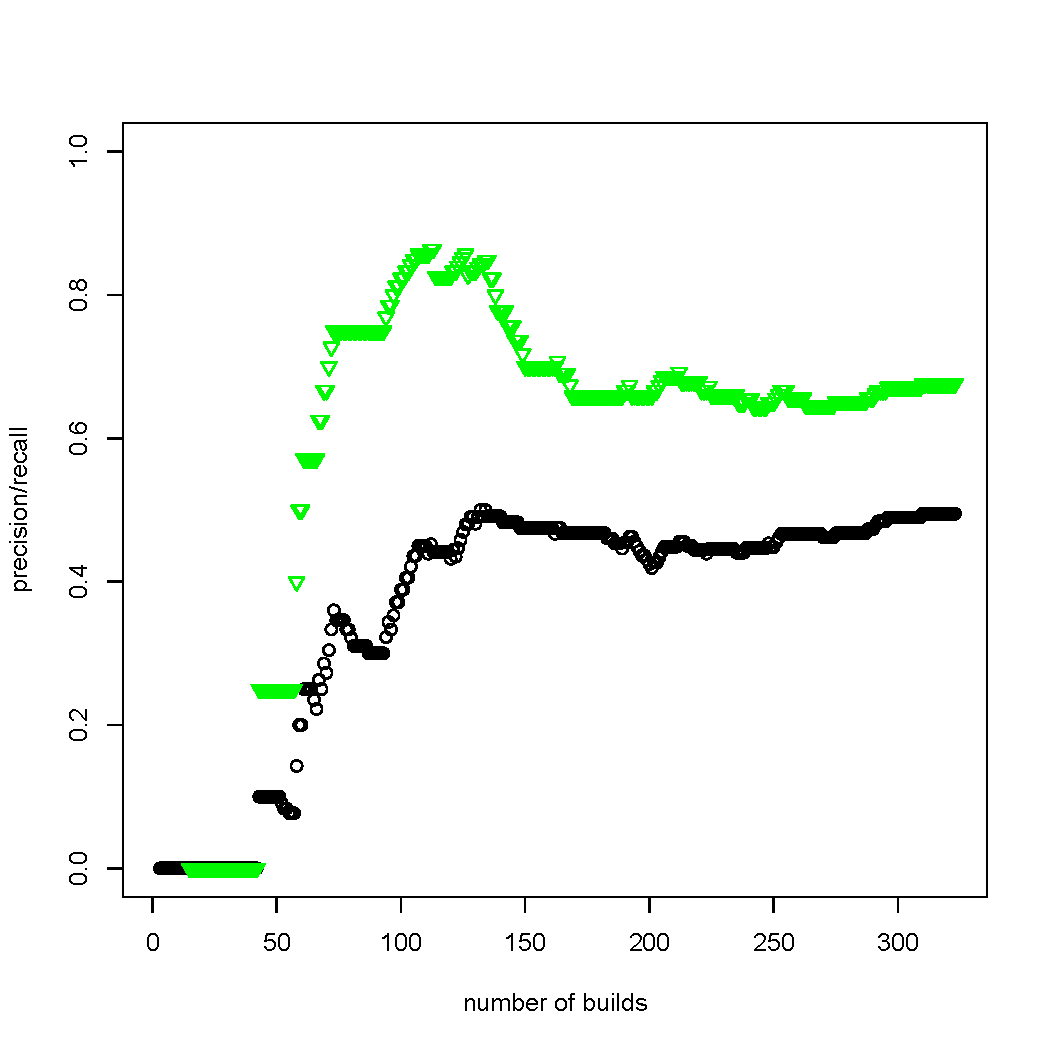
\includegraphics[width=\columnwidth]{precission-recall}
%\label{fig:prediction-svm}
%}
%\subfigure[Evaluation results from the Logistic Regression.] {
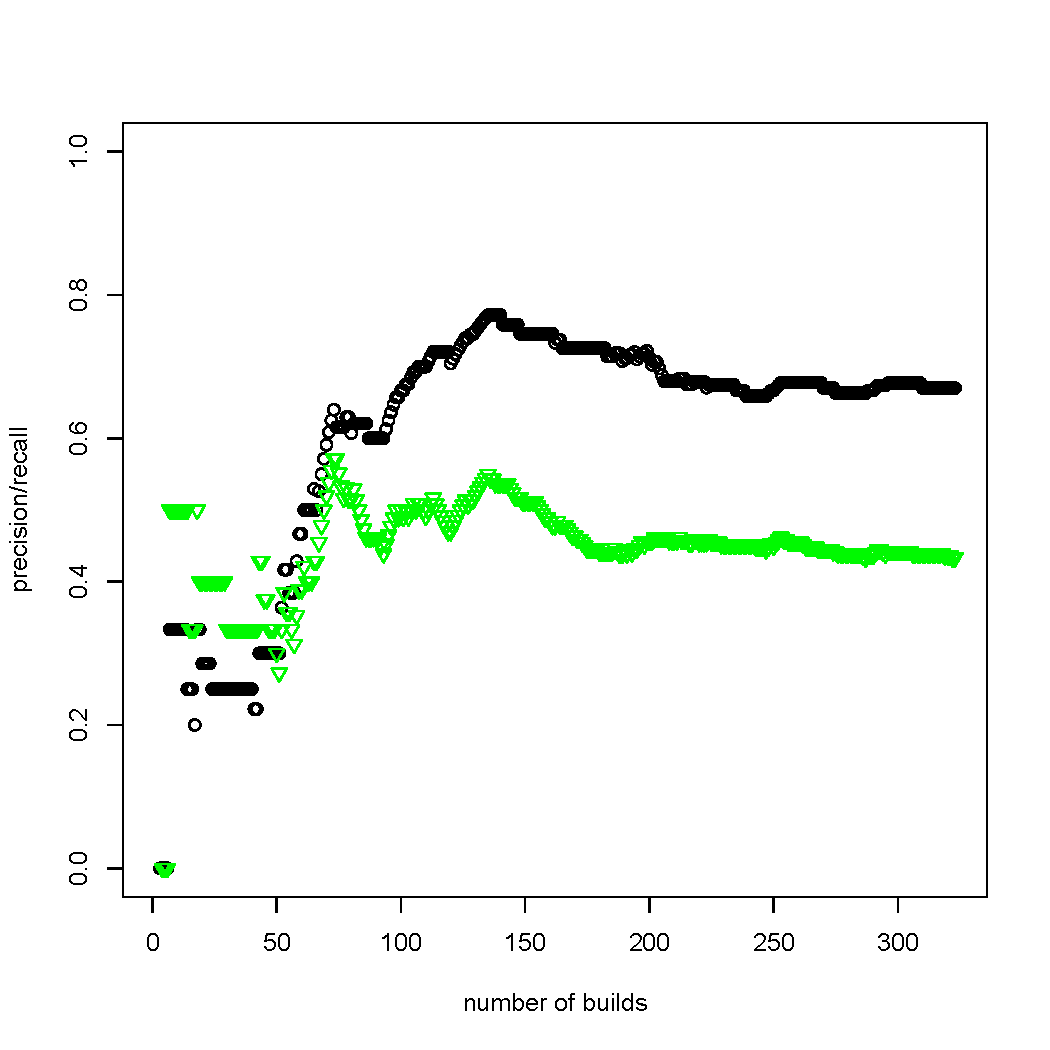
\includegraphics[width=\columnwidth]{precision-recall-logreg}
%\label{fig:prediction-logreg}
%}
\vspace{-25pt}
\caption{Precision (green) and recall (black) of the logistic regression.}
\label{fig:prediction}
\vspace{-10pt}
\end{figure}

To further validate our recommendations, we used the approach to generate a list of technical pairs for each of the 326 builds in our data. For any given build N we used the technical pairs as recommended by our approach from all the previous builds to build a logistical regression model predicting the outcome of build N. 
Applying this method to all builds yields Figure~\ref{fig:prediction} which shows the recall (black) and precision (green) values for the a logistical regression model used for prediction.
The recall and precision are cumulative at each point, including the prediction results obtained for the previous builds.
The logistical regression ended with a precision and recall value of $.43$ (median: $.45$) and $.67$ (median: $.67$) respectively, thus outperforming a random guess based on the ratio between failed and successful builds.
This further suggests that the recommendations that our approach identifies might prevent build failure. 

%WHAT DO THOSE NUMBERS FOR THE PREDICTION MEAN

In seeking explanations for the lack of communication in the RTC technical pairs found by our analysis, we were able to identify that most of these technical pairs consisted of developers belonging to
different teams. This confirms Naggappan et al.~\cite{nagappan:icse:2008}'s result that organizational distance predicts failures. Although the RTC team strongly emphasizes communication
regardless of team boundaries, it still seems that organizational distance had
an influence on its communication behaviour.

\emph{Threats to Validity.}
\label{sec:threats}
First, we performed our preliminary evaluation on one set of data, the Rational Team Concert\texttrademark\
repository, limiting the generalizability of our findings.
However, since the three months  we studied were directly before a major release of the project, 
we believe that this dataset is representative of a period in which lack of coordination (gaps) have the biggest impact on builds. Secondly, we assumed that every developer commenting on, or subscribed to, a work item reads all comments of that work item. 
By manual inspection of a selected number of work items, we found that developers who commented on a work item were aware of the other comments, confirming our assumption.

%Thirdly, Socio-technical dependencies may suffer from the combination of social and technical dependencies. 
%Social dependencies might not be related to the code changes the technical dependency was inferred from.
%Since the changes we used are directly linked to work item discussion we are confident that the vast majority of matches are appropriate.



\section{Conclusion and Next Steps}
Motivated by findings in the literature suggesting that socio-technical gaps increase build failure~\cite{kwan:tse:2011},
we hypothesized that these findings can be made actionable.
In this paper we proposed an approach that is capable of generating actionable knowledge that helps developers to prevent builds from failing.

Our results from the preliminary analysis with the RTC data indicate that 
the influence of developer pairs in a socio-technical gap on the build
failure was very high.
This knowledge can be used to improve the chances of the upcoming build to succeed.
Managers that oversee the work of several developers can initiate coordination between developers in technical pairs identified by our approach.
Similarly, a developer that is part of a technical pair in our recommendation can coordinate her work with her colleague to remove the risk posed by this open gap.

% We also found that historical project information about technical pairs and software
%builds can be used in a model that predicts the quality of upcoming builds.
%This means that if any one of the twenty most frequent failure related pairs was present in a social network of a build, the build had at least an 74\% chance to fail.

%PUT MORE

As a next step in our evaluation we have planned three follow up studies:
% MORE HERE be more explicit
(1) We want to examine the extent to which the technical pairs identified by our approach cause builds to fail. 
In our current approach we presented statistical evidence that the technical pairs relate to build failure, as a next step we will examine each technical pair and the failed builds it occurred in to determine if the technical pair actually cause the build to fail.
For example, we plan to identify the changes that broke a build and relate it back to the developers that made the changes and those that were affected by these changes.
%
%HOW CAN IT BE USED

(2) Develop a tool that implements our approach and provides real-time recommendations to the developer, and evaluated it with software practitioners. By comparing teams that do use the recommender system with those teams that do not, we plan on determining the effect the recommendations generated by our approach have on lowering the number of failed builds.

(3) Refine the definition of coordination and its needs, by both leveraging alternative conceptualizations of technical and social dependencies.
For example, we currently consider two developers having a technical dependency if they modified the same file, but plan to investigate alternative conceptualizations such as inferring technical dependencies from who uses code that has been modified.
\bibliographystyle{IEEEtran}
\bibliography{bib}

\end{document}


